\section{Chapter 5: Nuclear and renewables}

\subsection{Nuclear}

The global nuclear plant fleet is 450 reactors producing around 11\% of global
electricity.

Long opposition was caused by linking nuclear power to nuclear winter
post-nuclear war stories.

\textit{
Nuclear energy is a result of splitting uranium 235, an isotope found in rock
at about 2–3\% of uranium, depending on the origin of the ore. Most of the
balance is non-fissile uranium, U-238. Each split uranium 235 atom releases
heat, atomic fragments, and one or two neutrons can cause other uranium 235
atoms to also split. A consistent rate of radioactive decay of uranium 235
occurs in the core of a nuclear plant. This heat is used to make steam, turn a
turbine, and spin a generator. The reactor core is kept cool usually by
circulating water in the tower. Passively cooled power plants, which are not
yet commercially in operation, propose using gravity, density, or some other
physical process to ensure that cores of reactors are kept cool without the
need for an external energy source. Most nuclear power plants are either
boiling water reactors or pressured water reactors. The major difference is in
how the heat is transferred in the process of making steam.
}

Top two producers of uranium ore are Canada and Australia.

\subsection{Wind}

Power = $0.5 \times \rho \times C \times v^3 \times A_{\text{Sweep}}$

\begin{itemize}
	\item $V^3$: meters per second -- doubling of the wind results in
	eightfold increase in power
	\item $\rho = 1.2kg \cdot m^{-3}$ (kilograms per cubic meter)
	\item $A_S$: $m^2$ -- area swept by the blade
	\item $C$ -- efficiency coefficient depending on the turbine, usually
	between 0.4 and 0.5
\end{itemize}

Environmental toil: kills birds and bats.

\subsection{Solar}

PV problems:

\begin{itemize}
	\item require raw materials extracted from mines
	\item during installation, there can be impacts to ecosystems when
	utility-scale solar energy (USSE) projects are sited near wildlands or
	in sites that interfere with ecosystem processes
\end{itemize}

\textit{
PV modules generate electric current by
the photovoltaic effect, where incoming photons push electrons across a voltage.
While there are numerous other technologies that are colloquially called solar
power technologies, all non-PV solar technologies utilize the thermal energy
from the sun to heat liquids to produce hot water or to generate steam. PV
modules utilize photons to generate direct current and do not require moving
parts or steam like these other solar powered technologies.
}

A \textbf{photovoltaic module} is a device comprised of several photovoltaic
cells that is the principal unit of a photovoltaic array. A photovoltaic
module’s size is roughly 1 square meter.

Types of PV technologies:

\begin{itemize}
	\item \textbf{crystalline silicon} (90\% market share)
		\begin{itemize}
			\item mono-crystalline (10-20\% more efficient)
			\item multi-crystalline
		\end{itemize}
	\item \textbf{think films}
\end{itemize}

\textit{
Net metering is a simple model where prosumers generate their own
electricity, and only pay for what they import from the grid. In times of
excess, they can also export energy back to the grid for credit. Since the
Energy Policy Act of 2005, every public electrical utility is required to
offer net metering.
}

PV modules are the only renewable electricity source that can be readily
integrated into the built environment and atop residential and commercial
spaces and non-industrial zones.

\subsection{Hydropower}

Today, the world’s hydropower production is dominated by China, Canada, and
Brazil, with China producing 1,064 TWh.

Hydropower can change stream flows, increase turbidity, displace or lock-in
habitats, change fish migration patterns, degrade wilderness resources, and
increase erosion and landslides.

\subsection{Biofuels, biogases}

Biofuels are any organic matter available on a renewable or recurring basis.
This includes agricultural crops and trees; wood and wood wastes and residues;
plants (including aquatic plants); grasses; residues; fibers; and animal
wastes, municipal wastes, and other waste materials.

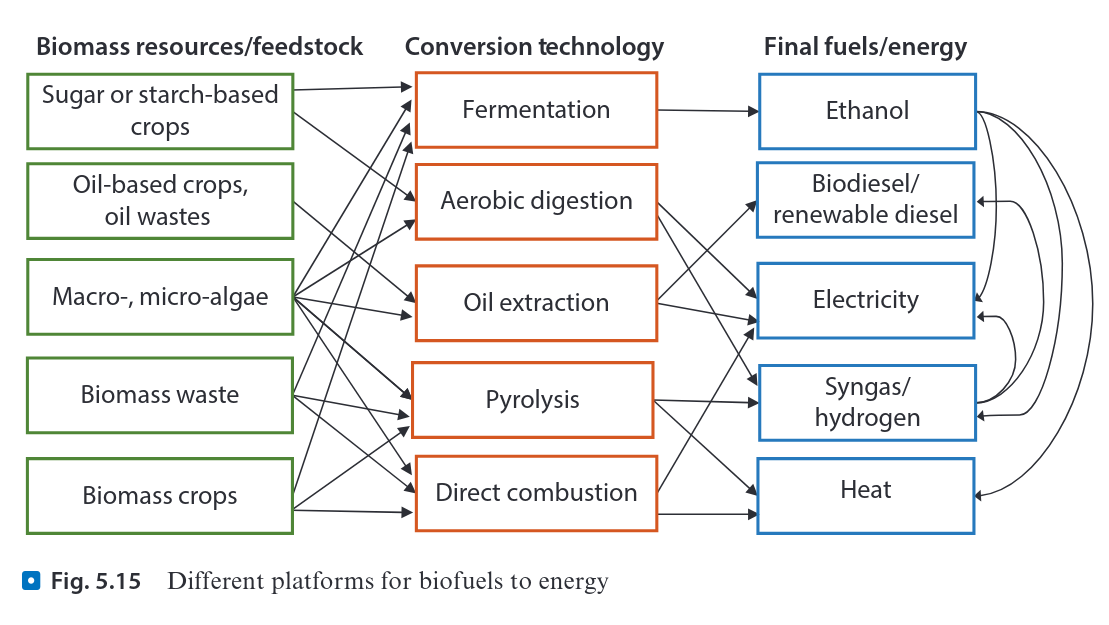
\includegraphics[scale=0.75\linewidth]{content/img/biomass.png}

Energy crops are high-yield production crop species.
These are higher energy content but more expensive to produce because they
require more inputs. They can roughly be divided into sugar crops, grains, and
oil seed crops.

\subsection{Geothermal}
